\Chapter{Existing and Developed Software}{An overview of \polsalt, \iraf, and \stops} %% custom chapter command (defined in preamble)

This chapter contains an overview of \polsalt\ (\S~\ref{sec:polsalt}) and the limitations faced during \polsalt\ wavelength calibrations (\S~\ref{subsec:polsalt_limits}), a brief overview of the \iraf\ tasks relevant to spectropolarimetric wavelength calibrations (\S~\ref{sec:iraf}), and an overview of \stops, the software developed to supplement the \polsalt\ reduction process (\S~\ref{sec:stops}). Finally, a discussion of the updated reduction process, an example of which may be found in Appendix~\ref{app:reduction}, is included (\S~\ref{sec:red_proc}).

% MARK: POLSALT
% http://salt-conference-2018.salt.ac.za/wp-content/uploads/2018/11/Groenewald.pdf
% https://saltworkshop2022.salt.ac.za/wp-content/uploads/2022/11/DG_polsalt_SALT_workshop_2022_finalversion.pdf
% https://github.com/saltastro/polsalt/wiki/Linear-Polarization-Reduction.--Beta-version#7-specpolfilterpy--compute-synthetic-filter-polarization-results-for-listed-filters
% https://github.com/saltastro/polsalt/wiki/
\section[\polsalt]{\polsalt\ - \glsxtrlong{POLSALT}} \label{sec:polsalt}

\begin{figure}[t]
    \centering
    \includegraphics[width = 0.8\textwidth]{figures/2_polsalt_gui.png}
    \caption{The layout of the \polsalt\ \gls{GUI}}
    \label{fig:polsalt_gui}
\end{figure}

\polsalt\ is the current reduction package being constantly developed and used within the \gls{SAAO}/\gls{SALT} research group as the official reduction pipeline for spectropolarimetric data taken using the \gls{SALT} \gls{RSS}.%
\footnote{\polsalt\ is made freely available via the \polsalt\ GitHub repository, available at \url{https://github.com/saltastro/polsalt}. It is strongly advised to follow the wiki for installation instructions.}
Newer versions of the software, aptly named the `beta version' (`version' 23 January 2020), include a \gls{GUI} as well as limited interactivity during key steps in the reduction process and was the version adapted in this study.%
\footnote{Installation files and instructions for the `beta version' utilizing the \gls{GUI} are available at \url{http://www.saao.ac.za/~ejk/polsalt/code/} in a TAR GZIP file.}

The steps that make up the \polsalt\ reduction pipeline include basic \gls{CCD} reductions, wavelength calibrations, background subtraction and spectral extraction, raw Stokes calculations, final Stokes calculations, and visualization of the results. Accurate reductions in each step are crucial for accurate results and thus briefly discussed. Further, detailed documentation for help with the reduction steps may be found at the \href{https://github.com/saltastro/polsalt/wiki}{GitHub wiki for \polsalt}.%
\footnote{The GitHub wiki for \polsalt\ is available at \url{https://github.com/saltastro/polsalt/wiki}.}

% MARK: Basic CCD reductions
\subsection{Basic CCD reductions}

Basic \gls{CCD} reductions are run via \textbf{imred.py} and apply the necessary basic reductions to the raw data before any calibrations may be applied. These corrections include overscan subtractions, gain corrections, crosstalk corrections, and mosaicking as well as attaching the bad pixel maps and pixel variance information. Files with basic reductions performed have ``mxgbp'' prepended to their names. As of February 2022, basic \gls{CCD} reductions are automatically run for all RSS spectropolarimetric observations as part of the default SALT basic reduction pipeline that is run each day.

% MARK: Wavelength calibrations
\subsection{Wavelength calibrations}

Wavelength calibration and cosmic-ray rejection is performed via \textbf{specpolwavmap.py} and separately calibrates the $O$- and $E$-beams, based on the arc frames, and applies a simple cosmic-ray rejection for all science frames. This step is interactive and allows the user to individually fit wavelength calibration maps to each beam. The importance of an accurate correlation between both beams has been touched on previously (\S~\ref{subsec:specpol_cal}) and will be further discussed in \S~\ref{subsec:polsalt_limits}. The wavelength calibrated results are saved as an additional extension to each science FITS file, which are prefixed with a ``w'', and the $O$- and $E$-beams of the extensions are split into their own sub-extensions.

% MARK: Background subtraction and spectral extraction
\subsection{Spectral extraction}

\begin{figure}[t]
    \centering
    % \includegraphics[width = 0.8\textwidth]{figures/2_polsalt_gui.png}
    \todo{Include \polsalt\ spectra extraction GUI}
    \caption{The layout of the interactive \polsalt\ \texttt{spectra extraction} \gls{GUI}}
    \label{fig:polsalt_gui_spec}
\end{figure}

Background subtraction and spectral extraction is run via \textbf{spec\-pol\-extract\_dev.py} which corrects for the beam-splitter distortion and tilt, performs sky subtraction, and extracts a one dimensional wavelength dependent spectrum for each beam sub-extension. This step is interactive and, using the brightest trace in the images, allows the user to define regions which span the wavelength axis and which define the background and trace regions for the sky subtraction and spectral extraction. Files with corrections applied are saved with ``c'' prepended to their names and files which contain the extracted one dimensional spectrum have ``e'' further prepended to their names.

% MARK: Raw Stokes calculations
\subsection{Raw Stokes calculations}

Raw Stokes calculations are performed via \textbf{specpolraw\-stokes\_dev.py} and identify waveplate pairs for which the intensity, $I$, and a `raw Stokes' signal, $S$, are calculated as:
\begin{equation}
    \begin{gathered}
        I = \frac{1}{2} (O_{1} + O_{2} + E_{1} + E_{2})\,,\rlap{\quad and}\\
        S = \frac{1}{2} \left[ \left( \frac{O_{1} - O_{2}}{O_{1} + O_{2}} \right) - \left( \frac{E_{1} - E_{2}}{E_{1} + E_{2}} \right) \right]\,,
    \end{gathered}\label{eq:polsalt_rawstokes}
\end{equation}
respectively. The raw Stokes signal is calculated as the normalized difference of the $O$- and $E$-beams, for a waveplate pair, taken perpendicular to one another. The files generated containing the raw Stokes information have a very specific naming style, which need not be discussed here but with most notably the pair of frames being used included in the file names.

% MARK: Final Stokes calculations
\subsection{Final Stokes calculations}

The Final Stokes calculations are performed via \textbf{specpolfinalstokes.py} and, using the waveplate pattern along with the raw Stokes signals, calibrate for polarimetric zero-point and waveplate efficiency calibrations and calculates the final Stokes parameters. Before the final Stokes calculations are performed, data culling is applied to the raw Stokes to eliminate outlier results which may arise due to, for example, atmospheric conditions. Data culling compares observation cycles against one another, compares the deviation of the means which estimate the systematic polarization baseline fluctuations (due to imperfections in repeatability), and performs a chi-squared analysis to eliminate outliers.

% MARK: Visualization
\subsection{Visualization}

\begin{figure}[t]
    \centering
    % \includegraphics[width = 0.8\textwidth]{figures/2_polsalt_gui.png}
    \todo{Include \polsalt\ visualisation GUI}
    \caption{The layout of the interactive \polsalt\ \texttt{visualisation} \gls{GUI}}
    \label{fig:polsalt_gui_vis}
\end{figure}

Plotting the results of the spectropolarimetric reduction process uses \textbf{specpolview.py} and generates a plot of the Intensity, Linear Polarization ($\%$), and Equatorial Polarization Angle ($\degr$) against a shared wavelength axis, as seen in Figure~\ref{fig:polsalt_plot}. This step is interactive and various options, such as the wavelength range, binning, etc., are available.

\begin{figure}[t]
    \centering
    \includegraphics[width = 0.8\textwidth]{figures/2_polsalt_plot.pdf}
    \caption{A typical plot resulting from the reduction process. Figure adapted from \citep{cooper_HEASA2022}}
    \label{fig:polsalt_plot}
\end{figure}

% MARK: Post-processing analysis
\subsection{Post-processing analysis}

Generally, the plot of the spectropolarimetric results is the stopping point for most reduction procedures as it contains or creates the desired results. However, additional tools exist which may be used after the polarization reductions, and which are not represented in the \gls{GUI}, namely, flux calibration and synthetic filtering.

Flux-calibrations are performed via \textbf{specpolflux.py} and are only intended for shape corrections of the spectrum. Additionally, the flux database file must exist for the standard observed and must be copied over to the working science directory.
% MARK: TODO: Flux Calibrations - errors in GUI - make 100\% sure about division error and notify Dani\'el

Synthetic filtering is calculated via \textbf{specpolfilter.py} and computes the synthetically filtered polarization results. The filters which can be synthesized are the Johnson $U$, $B$, and $V$ filter curves from the \gls{SALTICAM} filters, as well as the Cousins $R$ and $I$ filter curves, along with any user defined wavelength dependent throughput filter curves.

% MARK: Need for POLSALT
\subsection{Limitations of \polsalt\ and the Need for Supplementary Tools} \label{subsec:polsalt_limits}

% Why
The creation of supplementary tools for \polsalt\ spectropolarimetric reductions stemmed from the limitations of the wavelength calibration process and a need for a way to compare wavelength solutions across matching $O$ and $E$ polarization beams. The process of calibrating wavelength solutions using the \polsalt\ pipeline is time-consuming for the average user, and often results in unexpected crashes when receiving erroneous inputs or key presses. Due to the time-consuming process of recalibrating the wavelength solutions it is not feasible to perform the wavelength calibrations time and time again for any amount of reductions larger than a handful of observations.

% PG0300 reasoning
The prime motivation of finding an alternate method to wavelength calibrate \gls{SALT} spectropolarimetric data stemmed from a large backlog of unused data taken using the PG$0300$. The only arc available for the PG$0300$ with a close enough articulation and grating angle ($\sim 10.68\degr$ and $\sim 5.38\degr$, respectively) was \gls{SALT}'s Argon lamp which displayed sparse spectral features with large gaps over the wavelength range at these grating and articulation angles (Figure~\ref{fig:ar_arc_salt}). This often lead the \polsalt\ pipeline to create inconsistent wavelength solutions, or fail to create a wavelength solution altogether, since minor deviations of identified spectral features result in large deviations in regions with no spectral features. To only further compound the difficulty of the wavelength calibrations, the spectrum of the Ar arc lamp contains a partial overlap of a differing order at higher wavelengths and is thus not a purely free spectral range (\S~\ref{subsubsec:diff_grat}, Eq.~\ref{eq:grating_equation}).

% How
The chosen solution was to use a well established tool to perform the wavelength calibration - one which allows for rapid recalibrations as well as provides a familiar interface with which the user can analyze their wavelength solutions. \iraf\ provides this familiar environment and reliability, even when considering its age and \href{https://github.com/iraf-community/iraf}{limited community development}.

Unfortunately, \iraf\ is unable to natively parse the file structure implemented by \polsalt\ `as is' and formatting of the data structures are necessary for integration purposes. This restructuring works both ways as once the \iraf\ reductions are complete the format must be reformatted to match that of the \polsalt\ \texttt{wavelength calibration} output such that the reduction process may be completed in \polsalt.

Another option to perform the wavelength calibration is Python which allows for a more modern and flexible approach, but is not discussed here. What will be discussed, however, is the structure of the wavelength solutions created through Python to be later reintroduced to the \polsalt\ pipeline. The solutions must be stored such that the `$x$' and `$y$' orders of the solution, as well as all the coefficients ($C_{00}$ to $C_{xy}$) making up the solution, separated by new lines, are included. The only limitations to the names of the solution files is that they must make mention of the specific $O$- or $E$-beam as well as the wavelength solution type (e.g. `Chebyshev', `Legendre', etc.).

\begin{figure}[t]
    \centering
    \includegraphics[width = 0.98\textwidth]{figures/3_arc_spectrum.png}
    \caption{One of many Argon arc lamp spectra as provided by \gls{SALT} for line identification. Plot adapted from \gls{SALT}'s published Longslit Line Atlases (as of 2024), resized to fit within the document margins but otherwise unchanged.\protect\footnotemark}
    \label{fig:ar_arc_salt}
\end{figure}
\footnotetext{\protect\href{https://pysalt.salt.ac.za/lineatlas/plot_line_argon_lores.pdf}{`low resolution' Ar plot} sourced from \protect\url{https://astronomers.salt.ac.za/data/salt-longslit-line-atlas/}}

% MARK: IRAF
\section[\iraf]{\iraf\ - \glsxtrlong{IRAF}} \label{sec:iraf}

% What is IRAF and why necessary
\iraf\ is a collection of software designed specifically for the reduction and analysis of astronomical images and spectra. The software consists of many tasks which perform specific operations and which are grouped into relevant packages. Only a brief overview of the tasks will be provided here as every institute and individual has their own preferred wavelength calibration procedures and often use specific parameters for the various \iraf\ tasks (e.g. the order and type of the polynomial used in \texttt{identify}, etc.).

A useful \iraf\ task that will not be discussed but nevertheless deserves a mention is the \texttt{mkscript} task in the \texttt{system} package which allows a user to create and save a task along with the defined parameters as a file which can later be called as a script. It is instrumental as a scripting aid and is what allows \iraf\ its rapid recalibrations of the wavelength solutions.

Help documentation for any of the \iraf\ tasks may be found online under \url{https://iraf.net/irafdocs/} or through the \iraf\ \gls{CLI} through the \texttt{?} or \texttt{:.help} `cursor commands' when running interactive tasks.

For wavelength calibrations of spectropolarimetric observations taken with the \gls{SALT} \gls{RSS}, the relevant tasks, in order, are the \texttt{identify} and \texttt{reidentify} tasks located in the \texttt{noao.onedspec} package, and the \texttt{fitcoords} and optionally the \texttt{transform} tasks located under the \texttt{noao.twodspec.longslit} package. These tasks produce a two-dimensional wavelength solution and must each be run twice to find the wavelength solutions for both spectropolarimetric beams.

% MARK: Identify
\subsection{Identify}

The \texttt{identify} task is used to interactively determine a one-dimensional wavelength function across a chosen row of an arc exposure by identifying features in the spectrum with known wavelengths.%
\footnote{Help documentation for the \texttt{identify} task may be found at \url{https://astro.uni-bonn.de/~sysstw/lfa_html/iraf/noao.onedspec.identify.html}.}
The task creates the first approximation of the wavelength solution as well as a local database in which the solution is saved.%
\footnote{The structure of the \texttt{identify} database entry may be found at \url{https://iraf.net/irafdocs/formats/identify.php}.}
Both solution and database are built on in subsequent tasks, and it is therefore imperative that the initial solution is well-fit to minimize errors further down the calibration process.

The process of using \texttt{identify} consists of identifying known features spanning the entire wavelength range and then removing identified features which negatively impact the wavelength solution. A balance must be found between the number of identified features and parameters of the fit against the deviation of the fit from the known features.% RMS

% MARK: Reidentify
\subsection{Reidentify}

The \texttt{reidentify} task is used to run the \texttt{identify} task autonomously and repeatedly across the entirety of the arc exposure at a defined interval.%
\footnote{Help documentation for the \texttt{reidentify} task may be found at \url{https://astro.uni-bonn.de/~sysstw/lfa_html/iraf/noao.onedspec.reidentify.html}.}
The task uses the one-dimensional wavelength solution stored in the database created by the initial \texttt{identify} call and refits the previously identified points to match the new positions of the relevant spectral features. The task may fail based on a number of defined conditions, most common of which is the loss of features as the task moves further from the row at which the user ran \texttt{identify}.

When running \texttt{reidentify} non-interactively, it is recommended to set the \texttt{verbose} parameter to `\texttt{yes}' as this will provide immediate confirmation of whether the task quit early or not. Regardless of whether the task quit successfully or not, the newly defined wavelength solutions are appended to the local database following the \texttt{identify} task database format.

% MARK: Fitcoords
\subsection{Fitcoords}

The \texttt{fitcoords} task is used to combine the collection of one-dimensional wavelength solutions in the local database to a two-dimensional surface function.%
\footnote{Help documentation for the \texttt{fitcoords} task may be found at \url{https://astro.uni-bonn.de/~sysstw/lfa_html/iraf/noao.twodspec.longslit.fitcoords.html}.}
This surface function is the final two-dimensional wavelength solution and is what is needed to convert the \iraf\ formatted wavelength calibrated \gls{FITS} files back into the \polsalt\ format. The solution is stored in the local \iraf\ database and is the solution used by the \stops\ \texttt{join} method.%
\footnote{The structure of the \texttt{fitcoords} database entry may be found at \url{https://iraf.net/irafdocs/formats/fitcoords.php}.}

The process of using \texttt{fitcoords}, follows closely to that of \texttt{identify} and consists of examining the distribution of identified points and eliminating any points that \texttt{reidentify} may have misidentified. By eliminating outliers with bad residuals and modifying the two-dimensional surface function's type and degree, the overall error of the fit decreases, aligning more closely to what the `true' wavelength solution is.

% MARK: Transform
\subsection{Transform}

The \texttt{transform} task is the optional final step in the \iraf\ wavelength calibration process and is quick to run and easy to script.%
\footnote{Help documentation for the \texttt{transform} task may be found at \url{https://astro.uni-bonn.de/~sysstw/lfa_html/iraf/noao.twodspec.longslit.transform.html}.}
The task converts the (pixel, pixel) units of an exposure to (wavelength, pixel) units which allows for an immediate check whether the wavelength solution is consistent across the frame. Any general error in the wavelength solution may be spotted in the transformed images; ranging from minor errors, such as the arc exposure's arc lines or science exposure's sky lines not being straight across the columns of the frame, to more major errors, such as an incorrect wavelength solution skewing the exposure beyond recognition.

\begin{figure}[t]
    \centering
    % \includegraphics[width = 0.8\textwidth]{figures/2_polsalt_gui.png}
    \todo{Include poor and good transformed image examples}
    \caption{Examples of a terrible-, poorly-, and well-fit wavelength solution as presented by the \iraf\ \texttt{transform} task.}
    \label{fig:iraf_tran_eg}
\end{figure}

% MARK: STOPS
\section[\stops]{\stops\ - \glsxtrlong{STOPS}} \label{sec:stops}

\stops\ allows an alternate method for wavelength calibrations, namely \iraf, to be used instead of \polsalt's \texttt{wavelength calibration}. The parsing of \polsalt\ data into an \iraf\ usable format and the reformatting of the \iraf\ wavelength calibrated data back into a \polsalt\ usable format, referred to as \textit{splitting} and \textit{joining}, is performed by the \stops\ \texttt{split} and \texttt{join} methods, respectively.

Methods to verify the validity of the alternate wavelength calibrations were also added to \stops. The first of these methods checks the sky line wavelength ($x$) positions across the frame as well as the variation of the sky lines across the positional ($y$) axis of the frame, named \texttt{skyline}. The second of these methods checks the correlation of the $O$- and $E$-beams either within a given \gls{FITS} file or across multiple files (comparing only the $O$- and $E$-beams for each), named \texttt{correlate}. With these two additional methods, a user is able to verify that the wavelength solutions do not conflict across the $O$- and $E$-beams and that no unexpected deviations are included in the wavelength solutions.

Help for the \stops\ \gls{CLI} commands may be found either by running:
\begin{lstlisting}[language=bash]
$ python ~/STOPS --help
\end{lstlisting}
{\parskip=0pt or} in Listing~\ref{source:main}.
Help for the \stops\ specific mode commands may be found by running:
\begin{lstlisting}[language=bash]
$ python ~/STOPS [split|join|correlate|skylines] --help
\end{lstlisting}
{\parskip=0pt Finally}, help documentation for the \stops\ methods may be found within this section (Listings~\ref{doc:split} to \ref{doc:corr}) or in \S~\ref{app:code}.

% MARK: Split
\subsection{Splitting} \label{subsec:stops_split}

\lstinputlisting[
    language=python,
    style=sourceStyle,
    caption={The docstring for \textbf{split.py}},
    label=doc:split,
    linerange=split0-split1,
    gobble=4,
]{split.py}

% Why necessary
As mentioned previously, the format of the \gls{FITS} file created by \polsalt\ after basic \gls{CCD} reductions and the format expected by \iraf\ to be used for the wavelength calibrations are incompatible. Basic \polsalt\ \gls{CCD} reductions return \gls{FITS} files which contain a primary header along with extensions for the science, variance, and \gls{BPM} images. These extensions carry the image of the trace for both polarimetry beams (see Figure~\ref{fig:polsalt_pre_wav_cal}), the variance of the image, and a map of the pixels to be masked out, respectively.

\iraf\ is capable of dealing with multiple traces in an extension or lists of input files but is not as capable when dealing with multiple wavelength solutions contained in a single extension (as expected by the \polsalt\ \texttt{wavelength calibration}) or extensions containing sub-extensions (as expected by the \polsalt\ \texttt{spectral extraction}). To simplify the \iraf\ reduction procedure it was decided to separate the perpendicular polarization beams into their own files.

% What it does -> Primary focus
The files with \polsalt\ pre-reductions applied, namely \gls{FITS} files with an `mxgbp' prefix (\S~\ref{sec:polsalt}), are used as the starting point for the supplementary tool's \texttt{split} method. Running \texttt{split} finds all the \gls{FITS} files for wavelength calibration within the working directory, creates two empty \gls{HDU} structures for each sub-extension of the \gls{FITS} file, and appends all science and header data necessary for wavelength calibration to the relevant \gls{HDU} structure.

% Focus on minimizing changes and optimizing size
As the intent was always to parse the wavelength function back into \polsalt\ it was decided to keep these temporary \gls{FITS} files as small as possible. This is especially necessary when considering the amount of exposures that are taken for a single spectropolarimetric observation run, and then how the number of observations increases for long term studies.

\begin{figure}[t]
    \centering
    \includegraphics[width = 1.0\textwidth]{figures/3_OEsplit.pdf}
    \caption{The split $O$- and $E$-beams as handed to \iraf.}
    \label{fig:OE_split}
\end{figure}

% Any changes from how polsalt would do it
To aid the scripting of the \iraf\ wavelength calibration process, the \texttt{split} method also performs row cropping to exclude \gls{CCD} regions with no exposure and creates files listing the split $O$- and $E$-beam \gls{FITS} files to simplify the \iraf\ task inputs.%
\footnote{Row cropping was decided on as \iraf\ does not handle the empty rows well, specifically when it comes to the \texttt{reidentify} task.}
Otherwise, defaults, such as which row to split the beams along, were kept as close to the \polsalt\ pipeline as possible.

% MARK: Join
\subsection{Joining} \label{subsec:stops_join}

\lstinputlisting[
    language=python,
    style=sourceStyle,
    caption={The docstring for \textbf{join.py}},
    label=doc:join,
    linerange=join0-join1,
    gobble=4,
]{join.py}

As mentioned previously, the format of the \gls{FITS} file created by \iraf\ after wavelength calibrations and that expected by \polsalt\ for the \texttt{spectra extraction} are incompatible. A typical \gls{FITS} file expected by the \polsalt\ \texttt{spectra extraction} contains a primary header along with the various image extensions, the most notable extension being the newly added wavelength extension. All images contained within the extensions have the trace for both polarimetry beams split, as seen in Figure~\ref{fig:polsalt_post_wav_cal} and the headers of each extension updated.

All pieces necessary to recreate the \polsalt\ wavelength calibrated \gls{FITS} files exist once the \iraf\ procedure to generate the database entry for the two-dimensional wavelength solution is complete. The \texttt{join} method of the supplementary tools is used at this point and, once run, automatically creates the desired files.

Running \texttt{join} finds all the relevant \gls{FITS} and local database files necessary to run the \polsalt\ \texttt{spectra extraction}, creates an empty \gls{HDU} structure for each pair of matching spectropolarimetric beams, copies over the extensions and their respective image and header information, checks and corrects the trace splitting to best match that of \polsalt, appends a new extension and parses the database wavelength solutions into the \polsalt\ intensity-wavelength format, cleans the science extension for cosmic rays, and does some house-cleaning to align the finalized \gls{FITS} files to those created when using the `pure' \polsalt\ pipeline.

% update headers
% copy data, double check shape change
The \gls{FITS} files created by the \texttt{join} method and \polsalt\ pipeline's \texttt{wavelength calibration} methods are almost identical. The only difference between the \gls{FITS} files is the shape of the images stored within them, reflected also through specifically the `NAXIS2' header keyword, since \texttt{split} introduces a cropping. It was deemed unnecessary to reintroduce the cropped region as it is promptly discarded in the following \polsalt\ \texttt{spectra extraction} process and raises no issues when left out. Otherwise, both the \texttt{join} method and \polsalt\ \texttt{wavelength calibration} update the headers to reflect the new shape of the data and data type, through header keywords `CTYPE3' and `BITPIX', respectively.

% append new extensions
% How db converted to wav func
% parse and save wavelength functions as image
The wavelength extension is created entirely by \texttt{join} by appending a blank extension to the \gls{HDU} and filling the image pixels with their respective wavelength value. This is done entirely by \texttt{join} which parses the wavelength database file and creates a function which provides the corresponding wavelength when provided with a ($pixel$, $pixel$) position. This is used to fill the pixels of the wavelength extension with their respective wavelength, as seen in Figure~\ref{fig:pol_wav_ext}. Note that regions that fall outside the trace are masked by setting the wavelength extensions corresponding pixel value to $0$.

\begin{figure}[t]
    \centering
    \includegraphics[width = 1.0\textwidth]{figures/3_pol_wav_ext.pdf}
    \caption{The wavelength extension of a \gls{FITS} file ready to be handed back to the \polsalt\ pipeline. The color bar displays the wavelength in \AA as displayed by the $O$- and $E$-beam sub-extensions.}
    \label{fig:pol_wav_ext}
\end{figure}

% cosmic ray cleaning
The \texttt{join} method cleans the science extension of cosmic rays using the \texttt{lacosmic} python package which was specifically designed for this purpose and uses the L.A. Cosmic algorithm, based on Laplacian edge detection. The read noise and gain parameters used for cosmic ray cleaning were chosen based on the properties of the \gls{RSS}, while the rest were chosen following the publication and \hyperlink{http://www.astro.yale.edu/dokkum/lacosmic/pars.html}{suggestions} by the algorithm's creator, as well as the implementation of the algorithm in the python \texttt{ccdproc} package \citep{lacosmic,astroscrappy}. The chosen parameters work well for all but the worst of cosmic rays, as can be seen when comparing Figures~\ref{fig:OE_split} and \ref{fig:polsalt_post_wav_cal}.

% polsalt specific cropping (wav mask)
% mask wavelength using wollaston curve for polsalt `parsability'
% update BPM to reflect wavelength cropping
The wavelength extension is masked to remove any wavelength regions not calibrated for by \gls{SALT} as well as masked for the skewing of the trace introduced by the wollaston element. The masking of the wollaston skewing is necessary since \polsalt\ introduces a wollaston correction in the \texttt{spectra extraction} process. Finally, the \gls{BPM} extension is masked to reflect the valid wavelength calibrated regions for both spectropolarimetric beams and the files are saved with the \polsalt\ wavelength calibrated `wmxgbp' prefix.

\begin{figure}[t]
    \centering
    \includegraphics[width = 1.0\textwidth]{figures/3_post_wav_cal.pdf}
    \caption{A representative science extension of a \gls{FITS} file capable of being parsed by the \polsalt\ pipeline. The intensity of the $O$- and $E$-beam sub-extensions are displayed via the grayscale value at each pixel. Note the inclusion of regions of: solid black demarcating the chip gaps, horizontal stripes of high intensity demarcating the trace, and (curved) vertical stripes of high intensity demarcating the sky lines.}
    \label{fig:polsalt_post_wav_cal}
\end{figure}

% MARK: Skyline
\subsection{Sky line checks} \label{subsec:stops_skyline}

\lstinputlisting[
    language=python,
    style=sourceStyle,
    caption={The docstring for \textbf{skylines.py}},
    label=doc:skylines,
    linerange=sky0-sky1,
    gobble=4,
]{skylines.py}

\begin{figure}[t]
    \centering
    % \includegraphics[width = 0.8\textwidth]{figures/2_polsalt_gui.png}
    \todo{Include example of skyline result}
    \caption{The resultant output plot of the \stops\ \texttt{skylines} method.}
    \label{fig:stops_sky_eg}
\end{figure}

Sky line comparisons serve two unique yet interconnected services. Firstly, they naively transform the wavelength calibrated frames, without conserving flux, allowing the user confirmation of the variation of sky lines across the columns of the frame, and secondly, they compare the observed wavelength positions of the sky lines with the calibrated wavelength positions of the \gls{SALT} sky lines,%
\footnote{The first iteration of a sky line atlas is available at \url{https://astronomers.salt.ac.za/data/salt-longslit-line-atlas/}}
allowing confirmation of the wavelength solution at positions across the rows of the frame. The file used for skyline comparisons may be the \iraf\ \texttt{transform} \gls{FITS} file, which allows for flux conservation through the `\texttt{flux}' parameter.

The \texttt{skyline} method loads the wavelength calibrated files, transforms the frames (as described above) if the frame was not transformed by \iraf's \texttt{transform} method, divides out the continua, compares the cross-column sky lines to those of a single row, and compares the wavelength position of said sky lines to a list of sky lines known by \gls{SALT}.

Determining if there is an inaccuracy in the wavelength solution in the spatial ($y$, or vertical) axis is relatively straightforward as a perfect wavelength solution will remove any horizontal variation of the sky lines. Any horizontal deviation of the sky lines after transformation reflects a poor fit of the wavelength solution. Any vertical variation may be found through a quick visual inspection of a transformed frame, as mentioned previously, but may be inspected more thoroughly using the \texttt{skyline} method. As mentioned, the sky lines are averaged and compared to sky lines of a typical row. A wavelength solution exhibiting a poor fit across the spatial axis will display broader averaged sky lines than that of a relatively good fit.

As no features, other than the trace of sources exposed across a frame, exist that uniformly cover the wavelength ($x$, horizontal) axis of a typical frame, determining if the horizontal fit of the wavelength solution is more challenging. Thankfully, \gls{SALT} has published a sky line atlas which we may make use of. By first considering the spatial fit of the wavelength solution, it is ensured that the wavelength positions of all sky lines are well-defined. Comparisons may now be made to the wavelength positions measured by \gls{SALT}. Minor variations in the comparison of the sky lines are expected, but any uniform trends indicate an underlying poor fit across the wavelength axis of the wavelength solution. A poor horizontal fit is difficult to spot without supplementary tools and may have drastic adverse effect on the final polarization results.

% MARK: Correlate
\subsection{Cross correlation} \label{subsec:stops_correlate}

\lstinputlisting[
    language=python,
    style=sourceStyle,
    caption={The docstring for \textbf{cross\_correlate.py}},
    label=doc:corr,
    linerange=corr0-corr1,
    gobble=4,
]{cross_correlate.py}

\begin{figure}[t]
    \centering
    % \includegraphics[width = 0.8\textwidth]{figures/2_polsalt_gui.png}
    \todo{Include example of correlate result}
    \caption{The resultant output plot of the \stops\ \texttt{correlate} method.}
    \label{fig:stops_corr_eg}
\end{figure}

The \texttt{skyline} method allows for confirmation of a single wavelength solution, but has no means for comparing how the wavelength solutions of two polarization beams differ from each other. The difficulty arises in comparing the two spectra since variations between the two are expected and are what define the Stokes, and thus final polarization, results. The \texttt{correlate} method was created for this express purpose.

The \texttt{correlate} method loads the provided \gls{FITS} files created by the \polsalt\ \texttt{spectra extraction}, removes the continuum and separates the \gls{CCD} regions. The relevant, separated, \gls{CCD} regions are then cross correlated and any offset between the spectra may be plotted.

As the Stokes results, and thus final polarization results, are determined and are heavily influenced by the differences in the spectra of the different $O$ and $E$ beams, a direct comparison is not appropriate. Any observed unpolarized light, however, will reflect equally in both polarization beams and so the general trend of the two spectra may reasonably be expected to follow one another. Cross correlation of the two spectra for the different, $O$ and $E$, polarization beams allows for a comparison of the features within the spectra as a function of the wavelength displacement.

Sources under spectropolarimetric observation are often expected to vary over time and as such as the ratio of polarized to unpolarized light varies. The accuracy of correlation may decrease as features with differences in the polarized component of the polarization beams change. The differences in the features of the different spectra are often negligible when compared to the overall trend of the spectra and are generally only reflected in a change in the intensity of said features.

Cross correlation is useful when dealing with spectropolarimetric spectra as it allows a comparison of how well aligned the notable features of the spectra are wavelength-wise. Minor deviations between spectra weight the cross correlation less than the more prominent features, and therefore, cross correlation results acquired when using the \texttt{correlate} method more accurately reflect any general offset between polarization beams that may not necessarily be found when using the \texttt{skyline} method.

% MARK: General Reduction Procedure
\section{General Reduction Procedure}\label{sec:red_proc}

\begin{figure}[t]
    \centering
    \includegraphics[width = 0.8\textwidth]{figures/3_new_workflow.pdf}
    \caption{A general workflow for data reductions using a combination of \polsalt, \iraf, and the developed supplementary tools.}
    \label{fig:new_workflow}
\end{figure}

This section aims to provide a comprehensive discussion of the modified reduction procedure, an example of which is provided in Appendix~\ref{app:reduction}. As users all employ a variety of operating systems, language environments, and software setups, not much emphasis will be placed on how to get the software running or the managing of files: instead, the commands necessary to complete each step of the reduction process are discussed, assuming that the software is running as intended.

It is recommended to use \polsalt\ through the \gls{GUI} as it provides a user-friendly environment while also sequentially listing each step of the reduction process in a dropdown menu, as seen in Figure~\ref{fig:polsalt_gui}. Reductions are possible, however, purely through the \gls{CLI} using the \polsalt\ `beta' scripts.

% MARK: Pre-reductions
\subsection{\polsalt\ Pre-reductions}\label{subsec:reduc_pre}

\begin{figure}[t]
    \centering
    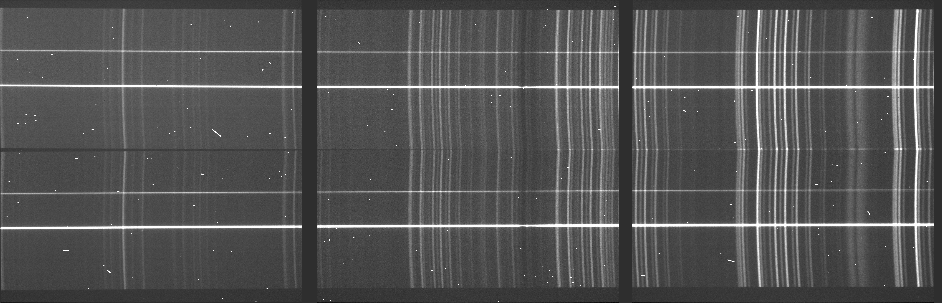
\includegraphics[width = 1.0\textwidth]{figures/3_pre_wav_cal.pdf}
    \caption{The science extension of a typical spectropolarimetric \acs{FITS} file taken with the \gls{SALT} \gls{RSS}, after basic \polsalt\ \gls{CCD} reductions have been completed.}
    \label{fig:polsalt_pre_wav_cal}
\end{figure}

The \polsalt\ reduction process requires a file structure such that the raw data received from \gls{SALT} is located in a folder labelled using the observing date with a sub-folder labelled raw, such as \texttt{YYYYMMDD/raw/}. This directory structure allows \polsalt\ to create a `working' directory named \texttt{YYYYMMDD/sci/} which contains all the files modified during the reduction process. Multiple reduction procedures using the same data may therefore be separated by simply renaming the \texttt{sci/} sub-folder.

The \polsalt\ \gls{GUI} may be launched by opening a \gls{CLI} and running Listing~\ref{code:polsalt_launch}. Once the window, depicted in Figure~\ref{fig:polsalt_gui}, has launched, ensure that the first two paths at the top of the window point to the \polsalt\ and working directories. The `raw image reduction' may then be selected from the dropdown and run.

Alternatively, if the data already includes `mxgbp' \gls{FITS} files in the \texttt{YYYYMMDD/sci/} working directory, a \gls{CLI} may be used to complete the initial pre-reductions using
\begin{lstlisting}[language=bash]
$ cd (*@<\textit{OBSDATE}>@*)/sci
$ conda activate salt
$ python ~/polsalt/scripts/reducepoldata_sc.py (*@<\textit{OBSDATE}>@*)
\end{lstlisting}
{\parskip=0pt which} will attempt to run the entire reduction process. The script may be quit once the \polsalt\ \texttt{wavelength calibration} \gls{GUI} opens and the rest of the reduction procedure followed.

% MARK: Wavelength Calibration
\subsection{Wavelength Calibration} \label{subsec:reduc_wav}

The wavelength calibrations may now be completed in \iraf. This section concerns the procedure for parsing the \gls{FITS} files to be read by \iraf\ and \polsalt\ as well as the relevant task names and methods to be run to complete the calibrations. A base working case of each of the tasks and methods are presented in Listings~\ref{code:stops_split}~-~\ref{code:stops_join}, but it should be noted that the art of wavelength calibration consists of modifying the parameters to achieve a good calibration function. This process depends heavily and varies greatly based on the user and as such not all use cases can be discussed herein.

% MARK: Prep for IRAF
\subsubsection{Preparing data for \iraf}

Splitting the data is presented in Lisiting~\ref{code:stops_split}. The \stops\ \texttt{split} method may take multiple parameters, as seen in \S~\ref{sec:stops}, but default parameters should be used where ever possible. The most notable parameters are the directory, which defaults to the current working directory of the \gls{CLI}, the split row, which defaults to \polsalt's default center row, and the save prefix, which defaults to `\texttt{obeam}' and `\texttt{ebeam}'. As an aside, the save prefix may be worth changing as, later in the reduction process, the \polsalt\ raw Stokes reductions indiscriminately selects files named \texttt{YYYYMMDD/sci/e*.fits}.

% MARK: IRAF wavelength calibrations
\subsubsection{\iraf\ wavelength calibrations}

The \iraf\ wavelength calibrations are performed using the tasks described in \S~\ref{sec:iraf}, namely \texttt{identify}, \texttt{reidentify}, \texttt{fitcoords}, and optionally \texttt{transform}. In general, these tasks are run directly in the \iraf\ terminal using:%
\footnote{Please see the \iraf\ help docs, available at \url{https://astro.uni-bonn.de/~sysstw/lfa_html/iraf/iraf.html}, on the relevant tasks for a comprehensive discussion of the parameters available.}
\begin{lstlisting}[language=bash]
cl> identify images
cl> reidentify reference images
cl> fitcoords images fitname
cl> transform images output fitname
\end{lstlisting}
{\parskip=0pt where} `images' refer to a list or file containing the \gls{FITS} files relevant to the task, `reference' refers to the \gls{FITS} file previously identified, `fitname' refers to the name to be used for the final two-dimensional wavelength solution, and `output' refers to the new file name for the transformed input images.

The interactive tasks take up the bulk of the reduction time as this is where the fine-tuning of the reduction is done, through the use of cursor (or colon) commands, which allow modification of the parameters mid-reduction. Task parameters may, however, be edited beforehand within the \iraf\ terminal using the \texttt{eparam} task, and optionally saved, and quit or run using a combination of \texttt{:w}, and \texttt{:q} or \texttt{:go} cursor commands, respectively.

The reduction process in Appendix~\ref{app:reduction}, namely Listings~\ref{code:iraf_id}~-~\ref{code:iraf_transform}, describes how to script the tasks for posterity. It is recommended to create an \iraf\ Command Language (cl) script for each task to keep track of which parameters were used and for simple recalibrations, but this is not strictly necessary. The scripts are created using the \texttt{mkscript} task which interactively asks for a task to script and parameters to use. Multiple tasks may be appended to an \iraf\ script, allowing for the parameters of both beams to be tracked. Running an \iraf\ script may be done by running:
\begin{lstlisting}[language=bash]
cl> cl < script_name.cl
\end{lstlisting}
{\parskip=0pt but} is not suggested for interactive scripts, which run best when simply copied from the \texttt{<.../>sci/script\_name.cl} file to the \iraf\ terminal.

% MARK: Post IRAF
\subsubsection{Preparing data for \polsalt}

The results of the wavelength calibrations may now be parsed back into the format expected by \polsalt\. Joining the separate beams with their respective wavelength solutions is once again performed in the \gls{CLI}following Listing~\ref{code:stops_join}.

Similar to the \texttt{split} procedure mentioned before, the \texttt{join} procedure has the same defaults defined and so the responsibility falls on a user to keep track of which defaults were changed, and to keep the parameters consistent between the two tasks. Note that \stops\ has logging implemented, see \S~\ref{sec:stops}, and so the onus of tracking the parameters may be passed on to a logging file.

% MARK: Skyline checks
\subsubsection{Sky line checks of the wavelength solution}

The optional \iraf\ \texttt{transform} task and \stops\ \texttt{skylines} method are used to confirm the wavelength solution across the frame, as described in \S~\ref{subsec:stops_skyline}, by comparing known and observed sky line wavelength positions.

The \texttt{skyline} method is run in the \gls{CLI} following Listing~\ref{code:stops_sky}. The difference in the flux conservation when \texttt{skyline} transforms the frames is discussed in \S~\ref{subsec:stops_skyline}. Otherwise, as with the rest of \stops, default parameters describe the overplotting behavior for the $O$- and $E$-beams, the skylines provided by \gls{SALT}, and the calculated variation of the wavelength axis of a frame.

A final reminder is made here about the clash of default naming schemes and the wildcard file collection performed by \polsalt. A simple wildcard `\texttt{mv}' move or `\texttt{rm}' remove command may be run in the \gls{CLI} to deal with the created split files used by \iraf. The remove command may be run using:
\begin{lstlisting}[language=bash]
$ rm obeam* ebeam*
\end{lstlisting}
{\parskip=0pt while} moving the files to a new subfolder may be done following Listing~\ref{code:gen_clean}.

The \texttt{correlate} method is run in the \gls{CLI} following Listing~\ref{code:stops_corr}. The input of the \texttt{correlate} method takes the output of the \polsalt\ \texttt{spectra extraction} and is thus only run thereafter, but is mentioned here as the completion of the \polsalt\ reductions is not discussed in much depth. If the user wishes to compare the $O$- and $E$-beams of a single file then only that image name is to be provided, otherwise it is assumed that the user wishes to compare the same polarization beam across each file provided.

% MARK: Complete reductions
\subsection{\polsalt\ Reduction Completion} \label{subsec:reduc_com}

Reductions may now be completed using \polsalt. The reduction process consists of correcting for the wollaston tilt, extracting the spectra, creating the Stokes files, and displaying the results. The `beta' version of \polsalt\ provides access to a \gls{GUI} but may also be handled entirely through a \gls{CLI} as scripts.

% MARK: POLSALT GUI
\subsubsection{\polsalt\ beta in a \gls{GUI}}

The reduction process using the \polsalt\ \gls{GUI} is completed by selecting and, when applicable, interactively modifying the reduction step through the interactive windows, one-by-one, from the \glspl{GUI} dropdown menu, as explained in Appendix~\ref{app:reduction} (pages~\pageref{code:stops_corr} onwards). As no commands are necessary, save for those to launch the \gls{GUI}, not much can be said of the reduction process. Excellent resources, created by the \gls{SALT}~/~\gls{SAAO} team, are available online for any queries about the reduction process using any version of \polsalt, including the \gls{GUI}.%
\footnote{See the official \href{https://github.com/saltastro/polsalt/wiki}{\polsalt\ wiki} or alternative online resources such as \href{https://saltworkshop2022.salt.ac.za/wp-content/uploads/2022/11/DG_polsalt_SALT_workshop_2022_finalversion.pdf}{\gls{SALT} workshop slides}.}

% Covering the \gls{CLI} implementation first, the wavelength solution needs to be applied to all the \gls{FITS} files and the tilt introduced by the wollaston prism must be corrected for. This is done through the command:
% \begin{lstlisting}[language=bash]
% $ python ~/polsalt/scripts/correct_files.py w*fits
% \end{lstlisting}
% {\parskip=0pt where} the `w*.fits' is a wildcard expression that lists the \gls{FITS} files that have a wavelength extension and returns it to the \polsalt\ script.

% Next, the spectra in each \gls{FITS} file are extracted using the command:
% \begin{lstlisting}[language=bash]
% $ python ~/polsalt/scripts/pol_extract.py c*.fits \
% > --yo A --ye B --dy C
% \end{lstlisting}
% {\parskip=0pt where} the center row of the spectra for the $O$- and $E$-beams, \texttt{A} and \texttt{B}, as well as the spectral width, \texttt{C}, are compulsory integer values. These may be found through \gls{FITS} viewing software such as ds9%
% \footnote{Available at \protect\url{https://sites.google.com/cfa.harvard.edu/saoimageds9}} or more manually through python.

% The Stokes files may then be calculated and created using the command:
% \begin{lstlisting}[language=bash]
% $ python ~/polsalt/scripts/pol_stokes.py
% \end{lstlisting}
% {\parskip=0pt which} automatically detects the \gls{FITS} files using the wildcards `e*fits' for raw Stokes and `*\_h*.fits' for the final Stokes calculations. The deletion of the \gls{FITS} files created in the supplementary \texttt{split} method may be deleted in the \texttt{join} method specifically to avoid this naming convention clash, but may also be avoided by providing an alternate default subscript to the supplementary methods.

% Finally, the results of the Stokes calculations may be viewed using the command:
% \begin{lstlisting}[language=bash]
% $ python polsalt/specpolview.py *_stokes.fits
% \end{lstlisting}
% {\parskip=0pt where} a file name, which may also use a wildcard, is provided as well as optional para\-meters to define the binning (\texttt{bin=[int]A} where [int] refers to an actual integer value), error bars (\texttt{errors=True|False}), choice of plot (\texttt{type=Ipt|Iqu} for unbinned intensity and either polarization percentage and polarization angle, or $Q$ and $U$ Stokes parameters), save options (\texttt{save=[text][plot] where either or both `text' and `plot' may be provided}), and a debug mode (\texttt{debug=False|True}).

% MARK: POLSALT CLI
\subsubsection{\polsalt\ beta in a \gls{CLI}}

The reduction script may be run using:
\begin{lstlisting}[language=bash]
$ python reducepoldata_sc.py YYYYMMDD
\end{lstlisting}
{\parskip=0pt which} will run the entire reduction process interactively without the need to select which process to run next. For the purposes of using the script alongside \iraf\ wavelength calibrations, a few changes must be made. The \texttt{imred} and \texttt{specpolwavmap} function calls before \texttt{specpolextract\_sc} should be commented out, since the raw images have already been processed and the wavelength calibrations were dealt with using \iraf.

The \polsalt\ beta \texttt{reducepoldata\_sc.py} copies a \texttt{script.py} file into the science working directory, `YYYYMMDD/sci/', which provides analysis scripts for analysis and modification of the \polsalt\ beta results. These tools consist of data culling for the final Stokes calculations, text and plot output, relative flux calibration corrections, and synthetic filtering of polarization results. The \polsalt\ analysis scripts may be run using:
\begin{lstlisting}[language=bash]
$ python script.py
\end{lstlisting}
{\parskip=0pt followed} by \texttt{specpolfinalstokes.py}, \texttt{specpolview.py}, \texttt{specpolflux.py}, or \texttt{specpol\-filter.py}, respectively, for the different analysis modes. A description of the use for each mode of the analysis script is available from \url{https://github.com/saltastro/polsalt/wiki/Linear-Polarization-Reduction.--Beta-version} and is exhaustive enough for general use, with the source code also publically available for in depth queries.

\todo{From appendix → Discuss - salt/py3 env, add polsalt GUI spectra extract and visualisation windows as images}
